\chapter{The Game Controller}
\label{cha:gameController}

The interpreter uses two handheld gamepads allowing user input for the running code to be acquired. Since two controllers can be connected at the same time, a multiplayer game can be developped using feedback from two different players. The interpreter does not check for keypresses itself, this is something the programmer has to poll for.
The controllers used are originally from a NES console. These controllers use SPI to communicate, and allow for more time to be spared on the console, since no development needs to be done anymore.

\section{Overview}
A total of 8 push buttons are present on the controller, all accessible by the user. Each button has two states, a pressed-state and a released-state. When the user presses a button the state changes form released to pressed and vice versa. The controller uses an SPI interface to allow communication with the game. The exact button states can be retreived once the interpreter is running.

\begin{figure}[h]
    \centering
	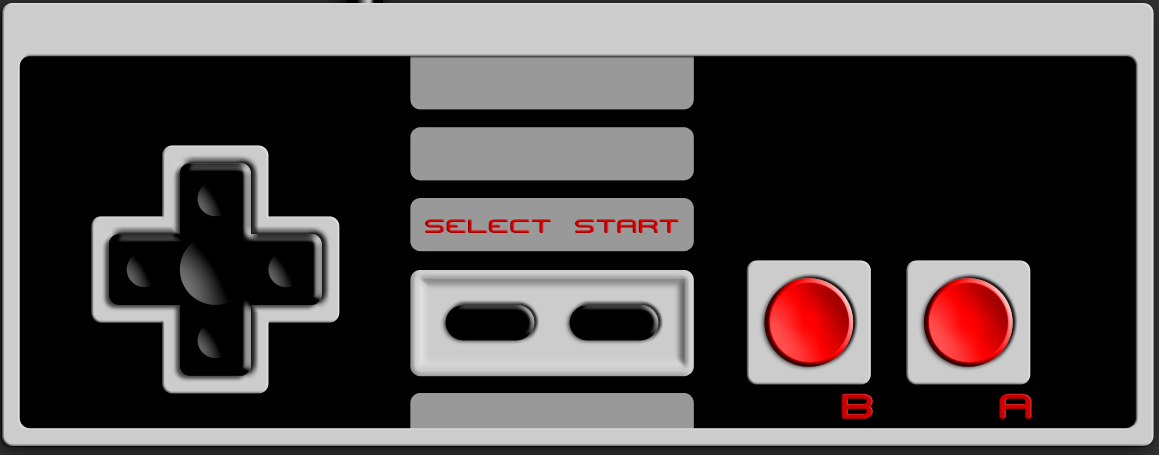
\includegraphics[width=0.7\textwidth]{GameController/GameControllerPicture.PNG}
    \caption{Game controller}\par
    \label{fig:GameController}
\end{figure}

\section{Buttons}
\subsection{D-Pad}
Four of these are formed as a D-Pad, a flat thumb-operated four-way directional control with one push button on each point, providing intuitive direction and steering capabilities, and should be used as such to provide a common interface for all developed games.

\subsection{Select, start}
In the center, the select and start button are located.
These should be used to start the game, pause it, allow menu navigation etc.
The start button should allow pausing the game at any point, pressing start again returns to the game.

\subsection{A and B}
Next to the select and start buttons are A and B located.
These two buttons are to be used in-game, providing interactivity with objects on the screen, and should not be used to pause or unpause the game at any time.
This can mean jumping on or over an obsacle, toggling a setting, opening a box\ldots

\section{Interface}
The controller is interfaced though a three-wire interface (with additional power and ground connections), equivalent to SPI.
A maximum of two controllers van be connected, and they are to be addressed as controller 0 and 1. The timing can be seen in this view:

\begin{figure}[h]
    \centering
	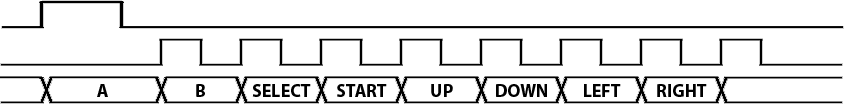
\includegraphics[width=\textwidth]{GameController/ControllerInterface.PNG}
    \caption{Interface timing of the controller}\par
    \label{fig:GameController}
\end{figure}